% ============================================================
%  arc.tex  –  Pipeline Architecture Figure (standalone)
%
%  Compile:
%    pdflatex arc.tex
%  Produces arc.pdf — a cropped figure ready for inclusion.
% ============================================================
\documentclass[tikz, border=10pt]{standalone}

\usepackage{amsmath,amssymb}
\usepackage{lmodern}
\usepackage[T1]{fontenc}

\usepackage{tikz}
\usetikzlibrary{
  shapes.geometric,
  arrows.meta,
  positioning,
  fit,
  backgrounds,
  calc,
  decorations.pathreplacing,
  shadows.blur
}

% ── colour palette ──────────────────────────────────────────
\definecolor{colInput}{HTML}{D6E8F7}   % soft blue  – inputs
\definecolor{colDRR}  {HTML}{C8EDE8}   % teal       – DRR generator
\definecolor{colPrep} {HTML}{FDE8CC}   % orange     – preprocessing
\definecolor{colSim}  {HTML}{E8D6F0}   % purple     – similarity
\definecolor{colCMA}  {HTML}{FDDCDC}   % red        – CMA-ES
\definecolor{colOut}  {HTML}{D4F0D4}   % green      – output
\definecolor{colBorder}{HTML}{555555}

% ── node styles ─────────────────────────────────────────────
\tikzset{
  %% generic box
  block/.style={
    draw=colBorder, line width=0.7pt,
    rounded corners=5pt,
    fill=#1,
    text width=2.8cm,
    minimum height=1.25cm,
    align=center,
    font=\small\sffamily,
    inner sep=5pt,
    blur shadow={shadow blur steps=4, shadow xshift=1pt,
                 shadow yshift=-1pt, shadow opacity=20}
  },
  block/.default=white,
  %% small annotation label
  ann/.style={font=\scriptsize\itshape\sffamily, text=gray!70!black},
  %% arrows
  arr/.style ={-{Stealth[length=7pt,width=5pt]}, thick, color=gray!60!black},
  darr/.style={-{Stealth[length=7pt,width=5pt]}, thick, color=gray!50!black,
               dashed},
  %% stage sub-box border
  cmaframe/.style={
    draw=red!45, dashed, line width=1pt,
    rounded corners=7pt, fill=red!4,
    inner sep=8pt
  },
  %% section header pill
  pill/.style={
    draw=#1!60, fill=#1!18, rounded corners=3pt,
    font=\bfseries\scriptsize\sffamily,
    inner sep=3pt, text=#1!70!black
  }
}

\begin{document}
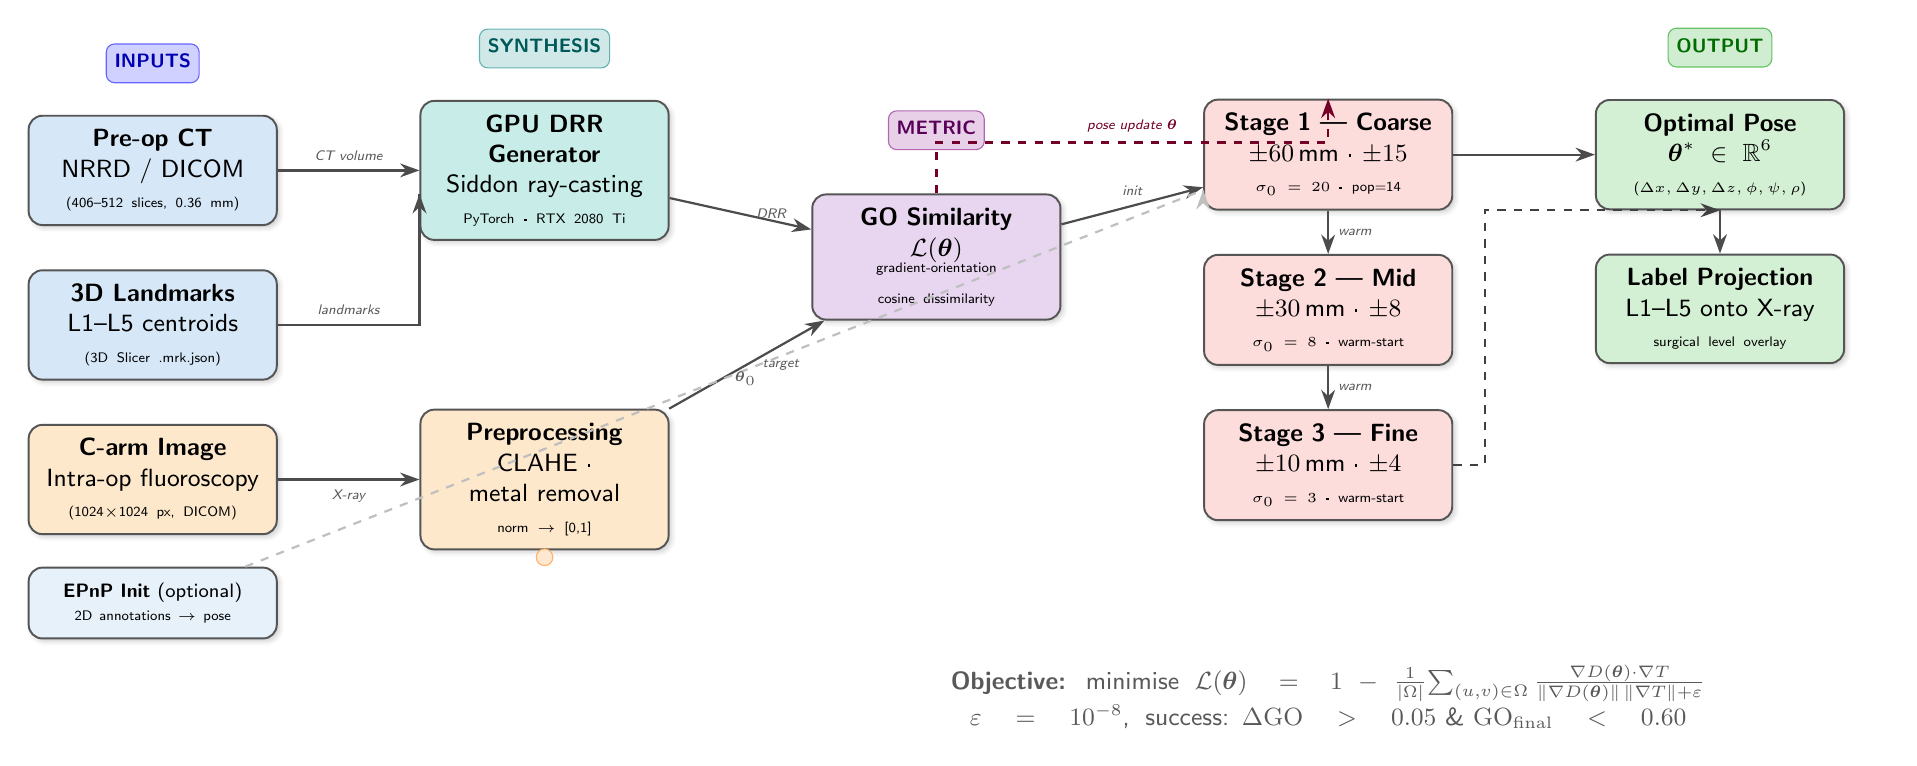
\begin{tikzpicture}[
  node distance = 0.6cm and 1.8cm,
]

% ════════════════════════════════════════════════════════════
% COLUMN 1 – INPUTS
% ════════════════════════════════════════════════════════════
\node[block=colInput] (ct) {%
  \textbf{Pre-op CT}\\
  \small NRRD / DICOM\\
  \tiny (406–512 slices, 0.36 mm)};

\node[block=colInput, below=0.55cm of ct] (lm) {%
  \textbf{3D Landmarks}\\
  \small L1–L5 centroids\\
  \tiny (3D Slicer .mrk.json)};

\node[block=colPrep, below=0.55cm of lm] (xray) {%
  \textbf{C-arm Image}\\
  \small Intra-op fluoroscopy\\
  \tiny (1024$\times$1024 px, DICOM)};

% section label
\node[pill=blue, above=0.4cm of ct, xshift=0pt]
     {\strut INPUTS};

% ════════════════════════════════════════════════════════════
% COLUMN 2 – PROCESSING
% ════════════════════════════════════════════════════════════
\node[block=colDRR, right=1.8cm of ct] (drr) {%
  \textbf{GPU DRR Generator}\\
  \small Siddon ray-casting\\
  \tiny PyTorch · RTX 2080 Ti};

\node[block=colPrep, right=1.8cm of xray] (pre) {%
  \textbf{Preprocessing}\\
  \small CLAHE · metal removal\\
  \tiny norm $\to$ [0,1]};

% vertical connector between drr and pre (visual guide)
\coordinate (midproc) at ($(drr.south)!0.5!(pre.north)$);

\node[pill=teal, above=0.4cm of drr, xshift=0pt]
     {\strut SYNTHESIS};
\node[pill=orange, above=0.4cm of pre, xshift=0pt, yshift=-2.4cm]
     {};

% ════════════════════════════════════════════════════════════
% COLUMN 3 – SIMILARITY
% ════════════════════════════════════════════════════════════
\node[block=colSim,
      right=1.8cm of drr,
      yshift=-1.1cm]          (sim) {%
  \textbf{GO Similarity}\\
  $\mathcal{L}(\boldsymbol{\theta})$\\
  \tiny gradient-orientation\\
  \tiny cosine dissimilarity};

\node[pill=violet, above=0.55cm of sim]
     {\strut METRIC};

% ════════════════════════════════════════════════════════════
% COLUMN 4 – CMA-ES STAGES
% ════════════════════════════════════════════════════════════
\node[block=colCMA, right=1.8cm of sim, yshift=1.3cm] (s1) {%
  \textbf{Stage 1 — Coarse}\\
  \small $\pm60$\,mm · $\pm15°$\\
  \tiny $\sigma_0=20$ · pop=14};

\node[block=colCMA, below=0.55cm of s1] (s2) {%
  \textbf{Stage 2 — Mid}\\
  \small $\pm30$\,mm · $\pm8°$\\
  \tiny $\sigma_0=8$ · warm-start};

\node[block=colCMA, below=0.55cm of s2] (s3) {%
  \textbf{Stage 3 — Fine}\\
  \small $\pm10$\,mm · $\pm4°$\\
  \tiny $\sigma_0=3$ · warm-start};

% dashed bounding box around CMA stages
\begin{scope}[on background layer]
  \node[cmaframe,
        fit=(s1)(s2)(s3),
        label={[pill=red, yshift=2pt]above:%
               \strut CMA-ES Optimisation}]
        (cmabox) {};
\end{scope}

% ════════════════════════════════════════════════════════════
% COLUMN 5 – OUTPUT
% ════════════════════════════════════════════════════════════
\node[block=colOut, right=1.8cm of s1] (pose) {%
  \textbf{Optimal Pose}\\
  $\boldsymbol{\theta}^* \in \mathbb{R}^6$\\
  \tiny ($\Delta x,\Delta y,\Delta z,\phi,\psi,\rho$)};

\node[block=colOut, below=0.55cm of pose] (overlay) {%
  \textbf{Label Projection}\\
  \small L1–L5 onto X-ray\\
  \tiny surgical level overlay};

\node[pill=green!60!black, above=0.4cm of pose]
     {\strut OUTPUT};

% ════════════════════════════════════════════════════════════
% ARROWS – forward flow
% ════════════════════════════════════════════════════════════
\draw[arr] (ct)    -- node[ann, above]{\tiny CT volume} (drr);
\draw[arr] (lm)    -| node[ann, near start, above]{\tiny landmarks}
                      ($(drr.west)+(0,-0.3)$) -- (drr);
\draw[arr] (xray)  -- node[ann, below]{\tiny X-ray} (pre);

\draw[arr] (drr)   -- node[ann, right, xshift=2pt]{\tiny DRR} (sim);
\draw[arr] (pre)   -- node[ann, right, xshift=2pt]{\tiny target} (sim);

\draw[arr] (sim)   -- node[ann, above]{\tiny init} (s1);
\draw[arr] (s1)    -- node[ann, right]{\tiny warm} (s2);
\draw[arr] (s2)    -- node[ann, right]{\tiny warm} (s3);

% s1 and s3 both feed into optimal pose
\draw[arr] (s1.east)  -- (pose.west);
\draw[darr] (s3.east) -- ++(0.4,0) |- (pose.south);

\draw[arr] (pose) -- (overlay);

% ════════════════════════════════════════════════════════════
% ARROW – feedback: pose update back to DRR
% ════════════════════════════════════════════════════════════
\draw[darr, color=purple!60!black, line width=0.9pt]
     (sim.north) -- ++(0, 0.65)
     -| node[ann, near start, above, color=purple!60!black]
        {\tiny pose update $\boldsymbol{\theta}$}
        (s1.north);

% ════════════════════════════════════════════════════════════
% ANNOTATION: EPnP init path (optional good init for Arjun)
% ════════════════════════════════════════════════════════════
\node[block=colInput!60, below=0.4cm of xray,
      text width=2.8cm, minimum height=0.9cm,
      font=\scriptsize\sffamily]
     (epnp) {%
       \textbf{EPnP Init} (optional)\\
       \tiny 2D annotations $\to$ pose};

\draw[darr, gray!50] (epnp) -- node[ann, right]{\tiny $\boldsymbol{\theta}_0$}
                                ($(s1.west)-(0,0.45)$) -- (s1);

% ════════════════════════════════════════════════════════════
% BOTTOM ANNOTATION BAR
% ════════════════════════════════════════════════════════════
\node[ann, below=1.4cm of cmabox, text width=14cm, align=center,
      font=\small\sffamily, text=gray!70!black]
     {%
       \textbf{Objective:}\;
       minimise\;
       $\mathcal{L}(\boldsymbol{\theta})
        = 1 - \frac{1}{|\Omega|}\!\sum_{(u,v)\in\Omega}
          \frac{\nabla D(\boldsymbol{\theta})\cdot\nabla T}
               {\|\nabla D(\boldsymbol{\theta})\|\,\|\nabla T\|+\varepsilon}$
       \quad $\varepsilon = 10^{-8}$,\;
       success: $\Delta\mathrm{GO}>0.05$ \& $\mathrm{GO}_\mathrm{final}<0.60$
     };

\end{tikzpicture}
\end{document}
